% Options for packages loaded elsewhere
\PassOptionsToPackage{unicode}{hyperref}
\PassOptionsToPackage{hyphens}{url}
\PassOptionsToPackage{dvipsnames,svgnames,x11names}{xcolor}
%
\documentclass[
  letterpaper,
  DIV=11,
  numbers=noendperiod]{scrartcl}

\usepackage{amsmath,amssymb}
\usepackage{iftex}
\ifPDFTeX
  \usepackage[T1]{fontenc}
  \usepackage[utf8]{inputenc}
  \usepackage{textcomp} % provide euro and other symbols
\else % if luatex or xetex
  \usepackage{unicode-math}
  \defaultfontfeatures{Scale=MatchLowercase}
  \defaultfontfeatures[\rmfamily]{Ligatures=TeX,Scale=1}
\fi
\usepackage{lmodern}
\ifPDFTeX\else  
    % xetex/luatex font selection
\fi
% Use upquote if available, for straight quotes in verbatim environments
\IfFileExists{upquote.sty}{\usepackage{upquote}}{}
\IfFileExists{microtype.sty}{% use microtype if available
  \usepackage[]{microtype}
  \UseMicrotypeSet[protrusion]{basicmath} % disable protrusion for tt fonts
}{}
\makeatletter
\@ifundefined{KOMAClassName}{% if non-KOMA class
  \IfFileExists{parskip.sty}{%
    \usepackage{parskip}
  }{% else
    \setlength{\parindent}{0pt}
    \setlength{\parskip}{6pt plus 2pt minus 1pt}}
}{% if KOMA class
  \KOMAoptions{parskip=half}}
\makeatother
\usepackage{xcolor}
\usepackage[left=1in,right=1in,top=1in,bottom=1in]{geometry}
\setlength{\emergencystretch}{3em} % prevent overfull lines
\setcounter{secnumdepth}{-\maxdimen} % remove section numbering
% Make \paragraph and \subparagraph free-standing
\ifx\paragraph\undefined\else
  \let\oldparagraph\paragraph
  \renewcommand{\paragraph}[1]{\oldparagraph{#1}\mbox{}}
\fi
\ifx\subparagraph\undefined\else
  \let\oldsubparagraph\subparagraph
  \renewcommand{\subparagraph}[1]{\oldsubparagraph{#1}\mbox{}}
\fi

\usepackage{color}
\usepackage{fancyvrb}
\newcommand{\VerbBar}{|}
\newcommand{\VERB}{\Verb[commandchars=\\\{\}]}
\DefineVerbatimEnvironment{Highlighting}{Verbatim}{commandchars=\\\{\}}
% Add ',fontsize=\small' for more characters per line
\usepackage{framed}
\definecolor{shadecolor}{RGB}{241,243,245}
\newenvironment{Shaded}{\begin{snugshade}}{\end{snugshade}}
\newcommand{\AlertTok}[1]{\textcolor[rgb]{0.68,0.00,0.00}{#1}}
\newcommand{\AnnotationTok}[1]{\textcolor[rgb]{0.37,0.37,0.37}{#1}}
\newcommand{\AttributeTok}[1]{\textcolor[rgb]{0.40,0.45,0.13}{#1}}
\newcommand{\BaseNTok}[1]{\textcolor[rgb]{0.68,0.00,0.00}{#1}}
\newcommand{\BuiltInTok}[1]{\textcolor[rgb]{0.00,0.23,0.31}{#1}}
\newcommand{\CharTok}[1]{\textcolor[rgb]{0.13,0.47,0.30}{#1}}
\newcommand{\CommentTok}[1]{\textcolor[rgb]{0.37,0.37,0.37}{#1}}
\newcommand{\CommentVarTok}[1]{\textcolor[rgb]{0.37,0.37,0.37}{\textit{#1}}}
\newcommand{\ConstantTok}[1]{\textcolor[rgb]{0.56,0.35,0.01}{#1}}
\newcommand{\ControlFlowTok}[1]{\textcolor[rgb]{0.00,0.23,0.31}{#1}}
\newcommand{\DataTypeTok}[1]{\textcolor[rgb]{0.68,0.00,0.00}{#1}}
\newcommand{\DecValTok}[1]{\textcolor[rgb]{0.68,0.00,0.00}{#1}}
\newcommand{\DocumentationTok}[1]{\textcolor[rgb]{0.37,0.37,0.37}{\textit{#1}}}
\newcommand{\ErrorTok}[1]{\textcolor[rgb]{0.68,0.00,0.00}{#1}}
\newcommand{\ExtensionTok}[1]{\textcolor[rgb]{0.00,0.23,0.31}{#1}}
\newcommand{\FloatTok}[1]{\textcolor[rgb]{0.68,0.00,0.00}{#1}}
\newcommand{\FunctionTok}[1]{\textcolor[rgb]{0.28,0.35,0.67}{#1}}
\newcommand{\ImportTok}[1]{\textcolor[rgb]{0.00,0.46,0.62}{#1}}
\newcommand{\InformationTok}[1]{\textcolor[rgb]{0.37,0.37,0.37}{#1}}
\newcommand{\KeywordTok}[1]{\textcolor[rgb]{0.00,0.23,0.31}{#1}}
\newcommand{\NormalTok}[1]{\textcolor[rgb]{0.00,0.23,0.31}{#1}}
\newcommand{\OperatorTok}[1]{\textcolor[rgb]{0.37,0.37,0.37}{#1}}
\newcommand{\OtherTok}[1]{\textcolor[rgb]{0.00,0.23,0.31}{#1}}
\newcommand{\PreprocessorTok}[1]{\textcolor[rgb]{0.68,0.00,0.00}{#1}}
\newcommand{\RegionMarkerTok}[1]{\textcolor[rgb]{0.00,0.23,0.31}{#1}}
\newcommand{\SpecialCharTok}[1]{\textcolor[rgb]{0.37,0.37,0.37}{#1}}
\newcommand{\SpecialStringTok}[1]{\textcolor[rgb]{0.13,0.47,0.30}{#1}}
\newcommand{\StringTok}[1]{\textcolor[rgb]{0.13,0.47,0.30}{#1}}
\newcommand{\VariableTok}[1]{\textcolor[rgb]{0.07,0.07,0.07}{#1}}
\newcommand{\VerbatimStringTok}[1]{\textcolor[rgb]{0.13,0.47,0.30}{#1}}
\newcommand{\WarningTok}[1]{\textcolor[rgb]{0.37,0.37,0.37}{\textit{#1}}}

\providecommand{\tightlist}{%
  \setlength{\itemsep}{0pt}\setlength{\parskip}{0pt}}\usepackage{longtable,booktabs,array}
\usepackage{calc} % for calculating minipage widths
% Correct order of tables after \paragraph or \subparagraph
\usepackage{etoolbox}
\makeatletter
\patchcmd\longtable{\par}{\if@noskipsec\mbox{}\fi\par}{}{}
\makeatother
% Allow footnotes in longtable head/foot
\IfFileExists{footnotehyper.sty}{\usepackage{footnotehyper}}{\usepackage{footnote}}
\makesavenoteenv{longtable}
\usepackage{graphicx}
\makeatletter
\def\maxwidth{\ifdim\Gin@nat@width>\linewidth\linewidth\else\Gin@nat@width\fi}
\def\maxheight{\ifdim\Gin@nat@height>\textheight\textheight\else\Gin@nat@height\fi}
\makeatother
% Scale images if necessary, so that they will not overflow the page
% margins by default, and it is still possible to overwrite the defaults
% using explicit options in \includegraphics[width, height, ...]{}
\setkeys{Gin}{width=\maxwidth,height=\maxheight,keepaspectratio}
% Set default figure placement to htbp
\makeatletter
\def\fps@figure{htbp}
\makeatother
\newlength{\cslhangindent}
\setlength{\cslhangindent}{1.5em}
\newlength{\csllabelwidth}
\setlength{\csllabelwidth}{3em}
\newlength{\cslentryspacingunit} % times entry-spacing
\setlength{\cslentryspacingunit}{\parskip}
\newenvironment{CSLReferences}[2] % #1 hanging-ident, #2 entry spacing
 {% don't indent paragraphs
  \setlength{\parindent}{0pt}
  % turn on hanging indent if param 1 is 1
  \ifodd #1
  \let\oldpar\par
  \def\par{\hangindent=\cslhangindent\oldpar}
  \fi
  % set entry spacing
  \setlength{\parskip}{#2\cslentryspacingunit}
 }%
 {}
\usepackage{calc}
\newcommand{\CSLBlock}[1]{#1\hfill\break}
\newcommand{\CSLLeftMargin}[1]{\parbox[t]{\csllabelwidth}{#1}}
\newcommand{\CSLRightInline}[1]{\parbox[t]{\linewidth - \csllabelwidth}{#1}\break}
\newcommand{\CSLIndent}[1]{\hspace{\cslhangindent}#1}

\usepackage{booktabs}
\usepackage{longtable}
\usepackage{array}
\usepackage{multirow}
\usepackage{wrapfig}
\usepackage{float}
\usepackage{colortbl}
\usepackage{pdflscape}
\usepackage{tabu}
\usepackage{threeparttable}
\usepackage{threeparttablex}
\usepackage[normalem]{ulem}
\usepackage{makecell}
\usepackage{xcolor}
\usepackage{fvextra}
\DefineVerbatimEnvironment{Highlighting}{Verbatim}{breaklines,commandchars=\\\{\}}
\DefineVerbatimEnvironment{OutputCode}{Verbatim}{breaklines,commandchars=\\\{\}}
\KOMAoption{captions}{tableheading}
\makeatletter
\makeatother
\makeatletter
\makeatother
\makeatletter
\@ifpackageloaded{caption}{}{\usepackage{caption}}
\AtBeginDocument{%
\ifdefined\contentsname
  \renewcommand*\contentsname{Table of contents}
\else
  \newcommand\contentsname{Table of contents}
\fi
\ifdefined\listfigurename
  \renewcommand*\listfigurename{List of Figures}
\else
  \newcommand\listfigurename{List of Figures}
\fi
\ifdefined\listtablename
  \renewcommand*\listtablename{List of Tables}
\else
  \newcommand\listtablename{List of Tables}
\fi
\ifdefined\figurename
  \renewcommand*\figurename{Figure}
\else
  \newcommand\figurename{Figure}
\fi
\ifdefined\tablename
  \renewcommand*\tablename{Table}
\else
  \newcommand\tablename{Table}
\fi
}
\@ifpackageloaded{float}{}{\usepackage{float}}
\floatstyle{ruled}
\@ifundefined{c@chapter}{\newfloat{codelisting}{h}{lop}}{\newfloat{codelisting}{h}{lop}[chapter]}
\floatname{codelisting}{Listing}
\newcommand*\listoflistings{\listof{codelisting}{List of Listings}}
\makeatother
\makeatletter
\@ifpackageloaded{caption}{}{\usepackage{caption}}
\@ifpackageloaded{subcaption}{}{\usepackage{subcaption}}
\makeatother
\makeatletter
\@ifpackageloaded{tcolorbox}{}{\usepackage[skins,breakable]{tcolorbox}}
\makeatother
\makeatletter
\@ifundefined{shadecolor}{\definecolor{shadecolor}{rgb}{.97, .97, .97}}
\makeatother
\makeatletter
\makeatother
\makeatletter
\makeatother
\ifLuaTeX
  \usepackage{selnolig}  % disable illegal ligatures
\fi
\IfFileExists{bookmark.sty}{\usepackage{bookmark}}{\usepackage{hyperref}}
\IfFileExists{xurl.sty}{\usepackage{xurl}}{} % add URL line breaks if available
\urlstyle{same} % disable monospaced font for URLs
\hypersetup{
  pdftitle={SDS 291 Final Project Report},
  pdfauthor={Miya Dang, Mia Tran, Alua Birgebayeva},
  colorlinks=true,
  linkcolor={blue},
  filecolor={Maroon},
  citecolor={Blue},
  urlcolor={Blue},
  pdfcreator={LaTeX via pandoc}}

\title{SDS 291 Final Project Report}
\author{Miya Dang, Mia Tran, Alua Birgebayeva}
\date{2025-04-28}

\begin{document}
\maketitle
\ifdefined\Shaded\renewenvironment{Shaded}{\begin{tcolorbox}[sharp corners, boxrule=0pt, interior hidden, frame hidden, borderline west={3pt}{0pt}{shadecolor}, enhanced, breakable]}{\end{tcolorbox}}\fi

\hypertarget{abstract}{%
\section{Abstract}\label{abstract}}

This study examines clinical predictors of mortality among patients with
heart failure using the Heart Failure Clinical Records Dataset from the
UCI Machine Learning Repository. The dataset contains detailed medical
profiles of 299 patients, including demographic, clinical, and
laboratory variables. Our objective was to build an interpretable and
statistically robust model that could identify individuals at elevated
risk of death during their follow-up period. After exploratory analysis
and variable selection through backward elimination using nested F-tests
(retention threshold: p \textless{} 0.1), we developed a logistic
regression model with five significant predictors: age, ejection
fraction, serum creatinine, serum sodium, and follow-up time. Model
diagnostics revealed no violations of key assumptions, and performance
metrics indicated strong predictive ability, with sensitivity of 81.3\%,
specificity of 79.3\%, accuracy of 79.9\%, and an AUC of 0.8935. These
results demonstrate that a small set of routinely collected clinical
variables can provide valuable insight into patient prognosis and
support early intervention in heart failure care.

\hypertarget{introduction}{%
\section{Introduction}\label{introduction}}

Heart failure is a chronic, progressive condition affecting over 64
million people globally and is a leading cause of morbidity and
mortality, particularly among older adults (Savarese \& Lund, 2017).
Timely identification of high-risk patients is critical in managing the
disease and preventing adverse outcomes. In clinical practice, easily
accessible indicators such as age, kidney function, and cardiac
performance are often used to guide care decisions. However, the
predictive value of these factors---especially in combination---requires
careful statistical modeling to ensure reliability and interpretability.

In this project, we seek to answer the following research question:
\textbf{\emph{Which clinical and demographic variables are most
predictive of mortality in patients with heart failure?}} To address
this, we utilized the Heart Failure Clinical Records Dataset, which
includes 13 variables measured during the follow-up of 299 patients. Our
primary outcome of interest is \texttt{DEATH\_EVENT}, a binary indicator
of whether the patient died during the follow-up period.

Prior research has explored predictors of heart failure outcomes using
machine learning and traditional statistical models. For example, Choi
et al. (Choi \& Lee, 2017) and Ahmad et al. (Ahmad et al., 2018)
identified low ejection fraction and elevated serum creatinine as
important mortality indicators, while Sulaiman et al. (Sulaiman et al.,
2020) highlighted the role of sodium levels in cardiac function. While
these studies provided clinical insights, many models lacked
transparency, and few incorporated robust diagnostic checks to assess
model assumptions and outliers.

To fill this gap, our study applies a multiple logistic regression
framework combined with backward elimination to select a parsimonious
set of predictors. We evaluate the model through statistical
diagnostics, including leverage, residuals, Cook's distance, and
multicollinearity analysis. We also assess model performance using
classification metrics and the ROC curve. By focusing on routinely
available variables and prioritizing interpretability, our goal is to
create a model that is both clinically meaningful and methodologically
sound---supporting real-world applications in early risk assessment for
heart failure patients.

\hypertarget{methods}{%
\section{Methods}\label{methods}}

\hypertarget{dataset-description}{%
\subsubsection{Dataset Description}\label{dataset-description}}

The dataset we analyzed in this study is the Heart Failure Clinical
Records Dataset, originally sourced from the UCI Machine Learning
Repository. It contains the medical records of 299 patients who
experienced heart failure, collected during their clinical follow-up
period. Each observation is a patient profile. The response variable,
DEATH\_EVENT, is a binary outcome indicating whether a patient died
during the follow-up period (1 = deceased, 0 = alive). All eleven
explanatory variables were initially considered, including demographic
factors, clinical profile, as well as laboratory blood tests
measurements. Details about each variable can be seen in Table 1. No
missing data were reported in the dataset.

\hypertarget{data-processing-and-exploratory-data-analysis}{%
\subsubsection{Data Processing and Exploratory Data
Analysis}\label{data-processing-and-exploratory-data-analysis}}

The dataset was imported into R, and all categorical variables were
recoded into factors.

An exploratory data analysis was performed using summary statistics and
visualizations. The median age of participants was 60 years (IQR:
51--70), and 32\% died during the follow-up period. The median serum
creatinine level was 1.10 mg/dL (IQR: 0.90--1.40), and the median
ejection fraction was 38\% (IQR: 30--45). Two boxplots were created to
compare the distributions of ejection fraction (\%) and serum creatinine
(mg/dL) by death event (Figure 1). These plots indicated that patients
who died tended to have lower ejection fractions and higher serum
creatinine levels, supporting the inclusion of these variables in
subsequent modeling.

\begin{table}

\caption{Summary of Heart Failure Dataset}
\centering
\begin{tabular}[t]{lc}
\toprule
\textbf{Characteristic} & \textbf{N = 299}\\
\midrule
age: age of the patient (years) & 60 (51, 70)\\
anaemia: decrease of red blood cells or hemoglobin (0 = No, 1 = Yes) & \\
\hspace{1em}0 & 170 (57\%)\\
\hspace{1em}1 & 129 (43\%)\\
creatinine\_phosphokinase: level of the CPK enzyme in the blood (mcg/L) & 250 (115, 582)\\
\addlinespace
diabetes: if the patient has diabetes (0 = No, 1 = Yes) & \\
\hspace{1em}0 & 174 (58\%)\\
\hspace{1em}1 & 125 (42\%)\\
ejection\_fraction: \% of blood leaving the heart at each contraction (\%) & 38 (30, 45)\\
high\_blood\_pressure: if the patient has hypertension (0 = No, 1 = Yes) & \\
\addlinespace
\hspace{1em}0 & 194 (65\%)\\
\hspace{1em}1 & 105 (35\%)\\
platelets: platelets in the blood (kiloplatelets/mL) & 262,000 (212,000, 304,000)\\
serum\_creatinine: level of serum creatinine in the blood (mg/dL) & 1.10 (0.90, 1.40)\\
serum\_sodium: level of serum sodium in the blood (mEq/L) & 137 (134, 140)\\
\addlinespace
sex: 0 = Woman, 1 = Man & \\
\hspace{1em}0 & 105 (35\%)\\
\hspace{1em}1 & 194 (65\%)\\
smoking: if the patient smokes (0 = No, 1 = Yes) & \\
\hspace{1em}0 & 203 (68\%)\\
\addlinespace
\hspace{1em}1 & 96 (32\%)\\
time: length of follow-up period (days) & 115 (73, 205)\\
DEATH\_EVENT: if the patient died during the follow-up period (0 = No, 1 = Yes) & \\
\hspace{1em}Alive & 203 (68\%)\\
\hspace{1em}Deceased & 96 (32\%)\\
\bottomrule
\multicolumn{2}{l}{\rule{0pt}{1em}\textsuperscript{1} Median (Q1, Q3); n (\%)}\\
\end{tabular}
\end{table}

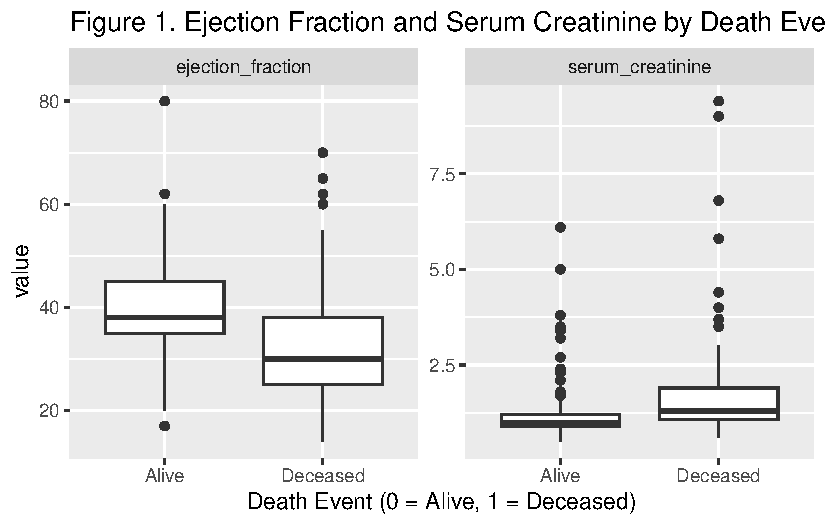
\includegraphics{SDS-291-final-project-report_files/figure-pdf/unnamed-chunk-3-1.pdf}

\hypertarget{variable-selection}{%
\subsubsection{Variable Selection}\label{variable-selection}}

To identify potential predictors of mortality, we applied backward
elimination to a full multiple logistic regression model containing 11
predictors. The selection process used nested F-tests with a retention
threshold of p \textless{} 0.1. Variables with the highest p-values were
removed sequentially until all remaining predictors had p-values below
the threshold. Variables removed sequentially included anaemia, smoking,
high\_blood\_pressure, diabetes, platelets, creatinine\_phosphokinase,
and sex. The final model retained five predictors: age,
ejection\_fraction, serum\_creatinine, serum\_sodium, and time.

The population form of the final model is defined as follows:

\[
\begin{aligned}
\text{logit}(P(\text{Deceased} = 1)) =\ & \beta_0 + \beta_1 \text{ (Age)} + \beta_2 \text{ (Eject Frac)} + \beta_3 \text{ (Serum Creatinine)} \\
& + \beta_4 \text{ (Serum Sodium}) + \beta_5 \text{ (Time)}
\end{aligned}
\]

Where:

\begin{itemize}
\item
  \(\text{logit}(P(\text{Deceased} = 1))\): The log-odds of the
  probability that the binary outcome ``Deceased'' equals 1.
\item
  \(\beta_0\): The intercept, the baseline log-odds of death when all
  predictors are zero. This is not particularly meaningful on its own,
  but it serves as a baseline for predictions.
\item
  \(\beta_1\): The slope for Age, the change in the log-odds of death
  for each 1 year increase in age, holding other variables constant.
\item
  \(\beta_2\): The slope for Ejection Fraction, the change in the
  log-odds of death for each 1\% increase in ejection fraction
  (percentage of blood leaving the heart at each contraction), holding
  other variables constant.
\item
  \(\beta_3\): The slope for Serum Creatinine, the change in the
  log-odds of death for each 1 mg/dL increase in the level of serum
  creatinine in the blood, holding other variables constant.
\item
  \(\beta_4\): The slope for Serum Sodium, the change in the log-odds of
  death for each 1 mEq/L increase in the level of serum sodium in the
  blood, holding other variables constant.
\item
  \(\beta_5\): The slope for Time, the change in the log-odds of death
  for each 1 day increase in the length of the follow-up period, holding
  other variables constant.
\end{itemize}

\begin{table}[H]
\centering
\caption{Coefficient Estimates from Final Model}
\centering
\begin{tabular}[t]{lcccc}
\toprule
  & Estimate & Std. Error & t value & Pr(>|t|)\\
\midrule
(Intercept) & 9.4930 & 5.4058 & 1.7561 & 0.07907\\
age & 0.0425 & 0.0150 & 2.8255 & 0.00472\\
ejection\_fraction & -0.0734 & 0.0158 & -4.6518 & 0.00000\\
serum\_creatinine & 0.6860 & 0.1740 & 3.9415 & 0.00008\\
serum\_sodium & -0.0646 & 0.0384 & -1.6822 & 0.09254\\
time & -0.0209 & 0.0029 & -7.1657 & 0.00000\\
\bottomrule
\end{tabular}
\end{table}

\hypertarget{model-diagnostics-influential-points-and-model-assumptions}{%
\subsubsection{Model Diagnostics: Influential Points and Model
Assumptions}\label{model-diagnostics-influential-points-and-model-assumptions}}

We then investigated influential observations and assessed model
assumptions to ensure the reliability of our logistic regression model.
To identify unusual points, we examined leverage, studentized residuals,
and Cook's distance for all observations. Observations with leverage
values greater than \(\frac{2(k+1)}{n}\) and studentized residuals
\(> 2\) or \(< -2\) were flagged as potentially influential. Initially,
we used a threshold of \(\frac{4}{n}\) for Cook's distance, which
flagged 29 observations as influential, which is nearly 10\% of the
dataset. However, upon visual inspection of the Cook's distance plot,
most of these points clustered closely with the rest of the data and did
not appear to exert a disproportionate influence on the model. Only
three observations (rows 132, 218, and 229) were clearly distant from
the majority, with Cook's distance values exceeding 0.05. We therefore
adopted 0.05 as a more appropriate threshold and focused on these three
points, which were also consistently flagged across all diagnostic
metrics. Further inspection revealed that these three observations had
unusually high serum creatinine levels (6.1, 9.0, and 5.0). While these
values are high, they are not uniquely extreme within the dataset as
several other cases also exhibited elevated serum creatinine levels
above 3.0. These high values are clinically plausible and likely reflect
cases of severe kidney dysfunction, a condition frequently associated
with heart failure and increased mortality risk. Therefore, there is no
indication that these values are due to data entry or recording errors.
Additionally, serum creatinine remained a statistically significant and
clinically meaningful predictor in both the original model and the clean
model that excluded them, with consistent effect sizes and p-values.
Importantly, model performance metrics such as AIC, deviance, and
coefficient estimates did not change substantially after excluding these
observations. Based on this evidence, we concluded that the flagged
cases represent valid and meaningful variation in the data and chose to
retain them in the final model to maintain the integrity and
generalizability of our findings.

We assessed multicollinearity among our predictors by calculating
Variance Inflation Factors (VIFs). All VIFs fell between 1.03 and 1.13,
indicating minimal correlation among the covariates and reassuring us
that our coefficient estimates are stable and interpretable. Next, we
generated a deviance‐residual plot to evaluate model fit and again
identify any unusual observations. The residuals are scattered randomly
around zero without any clear pattern across the observation index,
suggesting the model does not systematically over- or under-predict in
different regions of the data. Moreover, all deviance residuals lie
within the range of --3 to +3, and there are no points that stand apart
from the main cluster. Together, these diagnostics confirm that our
model assumptions hold and that no extreme outliers warrant removal.

\hypertarget{model-performance}{%
\subsubsection{Model Performance}\label{model-performance}}

We evaluated the model's performance using sensitivity, specificity,
accuracy, and the area under the ROC curve (AUC). To reduce the risk of
missing actual mortality cases, we selected a lower classification
threshold of \(\pi_0 = 0.3\), prioritizing sensitivity over specificity.
Using this cutoff, we calculated the corresponding performance metrics
to assess how well the model distinguishes between patients who survived
and those who died.

\begin{itemize}
\item
  Sensitivity (0.8125): The model correctly identifies 81.3\% of
  individuals who died (DEATH\_EVENT = 1). This indicates strong
  performance in detecting patients at high risk of death, which is
  especially important in clinical settings where failing to identify
  at-risk patients could have serious consequences.
\item
  Specificity (0.7931034): The model correctly classifies 79.3\% of
  individuals who survived (DEATH\_EVENT = 0). This means it is also
  reasonably effective at minimizing false positives, avoiding
  misclassifying living patients as deceased.
\item
  Accuracy (0.7993311): The model achieves an overall accuracy of
  approximately 79.9\%, meaning it correctly classifies nearly 80\% of
  all cases, whether alive or dead. This suggests strong overall
  predictive ability.
\item
  AUC (0.8935242): The model has excellent discriminative ability, with
  an AUC of 0.8935. This indicates that it can distinguish between
  patients who died and those who survived substantially better than
  random chance, and approaches the performance of a highly reliable
  classifier.
\end{itemize}

\hypertarget{results}{%
\section{Results}\label{results}}

The final analysis included all 299 patients in the dataset. Although
three observations were flagged as potentially influential, they were
retained in the model after further diagnostics. Out of these 299
patients, 32\% died during the follow-up period.

The response variable, DEATH\_EVENT, indicates whether a patient died
during the follow-up period (1 = deceased, 0 = alive). The explanatory
variables retained in the final model were age (in years), ejection
fraction (percentage of blood leaving the heart per contraction), serum
creatinine (mg/dL), serum sodium (mEq/L), and time (length of follow-up
in days). These variables were selected through backward elimination
using nested F-tests with a retention threshold of p \textless{} 0.1.
The table below summarizes the estimated odds ratios, 95\% confidence
intervals, and p-values for each predictor in the model.

\begin{longtable}[t]{lrrrr}
\caption{Final Model: Odds Ratios and 95\% Confidence Intervals}\\
\toprule
Predictor & Odds Ratio & 95\% CI (Low) & 95\% CI (High) & p-value\\
\midrule
Age & 1.043 & 1.014 & 1.076 & 0.005\\
Ejection Fraction & 0.929 & 0.899 & 0.957 & 0.000\\
Serum Creatinine & 1.986 & 1.421 & 2.874 & 0.000\\
Serum Sodium & 0.937 & 0.868 & 1.011 & 0.093\\
Follow-up Time & 0.979 & 0.973 & 0.985 & 0.000\\
\bottomrule
\end{longtable}

Each predictor in the final model had a clear association with the
probability of death.

\begin{itemize}
\item
  \textbf{Age}: Each additional year increased the odds of death by
  approximately 4.3\% (OR = 1.043, 95\% CI: {[}1.014, 1.076{]}, p =
  0.005).
\item
  \textbf{Ejection Fraction}: Each 1\% increase reduced the odds of
  death by 7.1\% (OR = 0.929, 95\% CI: {[}0.899, 0.957{]}, p \textless{}
  0.001).
\item
  \textbf{Serum Creatinine}: Each 1 mg/dL increase more than doubled the
  odds of death (OR = 1.986, 95\% CI: {[}1.421, 2.874{]}, p \textless{}
  0.001).
\item
  \textbf{Serum Sodium}: While not statistically significant, the odds
  ratio suggests a 6.3\% decrease in risk per unit increase (OR = 0.937,
  95\% CI: {[}0.868, 1.011{]}, p = 0.093).
\item
  \textbf{Follow-up Time}: Each additional day of follow-up was
  associated with a 2.1\% decrease in the odds of death (OR = 0.979,
  95\% CI: {[}0.973, 0.985{]}, p \textless{} 0.001).
\end{itemize}

To evaluate model performance, we selected a classification threshold of
\(\pi\) = 0.3 to prioritize sensitivity. The model correctly identified
81.3\% of patients who died (sensitivity) and 79.3\% of patients who
survived (specificity). Overall classification accuracy was 79.9\%. The
area under the ROC curve (AUC) was 0.8935, indicating excellent
discriminative ability.

Figure 1 shows boxplots of ejection fraction and serum creatinine by
survival outcome. Patients who died had noticeably lower ejection
fractions and higher creatinine levels, reinforcing their inclusion in
the final model.

These findings address our research question by identifying five
routinely available variables that effectively predict mortality among
patients with heart failure.

\hypertarget{discussion}{%
\section{Discussion}\label{discussion}}

This study set out to answer the question: \emph{Which variables best
predict death during the follow-up period after a heart failure
diagnosis?} Using logistic regression and backward elimination, we
identified five key predictors: age, ejection fraction, serum
creatinine, serum sodium, and follow-up time.

Our results show that these variables are strong predictors of
mortality. Older patients, those with lower ejection fractions, and
those with higher serum creatinine levels were significantly more likely
to die during follow-up. While serum sodium was not statistically
significant at the 5\% level (p = 0.093), its clinical relevance and
borderline confidence interval supported its inclusion. Patients with
longer follow-up times were less likely to die, suggesting that time
itself may reflect survival resilience.

These findings directly answer our research question and are supported
by both statistical metrics and clinical interpretability. As shown in
Table 3, odds ratios for the significant predictors were all in
directions consistent with medical expectations. Figure 1 further
reinforced these relationships, visually demonstrating that patients who
died had lower ejection fractions and higher serum creatinine. Model
performance metrics, including a high AUC (0.8935), sensitivity
(81.3\%), and specificity (79.3\%), indicate that the model performs
well as a classification tool.

Despite these strengths, our analysis has several limitations. First,
the dataset contains only 299 observations, which limits the
generalizability of our findings. All data came from a single source,
and we do not have access to variables such as treatment type,
comorbidities, or socioeconomic status. These missing factors may
introduce omitted variable bias. Additionally, our model assumes
linearity in the log-odds and does not explore potential interactions or
non-linear effects.

Still, the study has notable strengths. The final model is
interpretable, relies on common clinical measures, and passed all major
diagnostic checks (e.g., residuals, Cook's distance, VIFs). Our variable
selection process used nested F-tests, and we retained cases flagged as
influential only after confirming they did not distort results. These
decisions reflect a balance between statistical rigor and real-world
applicability.

In summary, this analysis provides strong evidence that five routine
clinical measures can meaningfully predict death in heart failure
patients. However, our conclusions are specific to the dataset at hand
and should not be generalized without further validation. These findings
offer a starting point for clinicians or researchers seeking to build
early warning tools using accessible patient data.

\hypertarget{data-analysis-appendix}{%
\section{Data Analysis Appendix}\label{data-analysis-appendix}}

\hypertarget{import-dataset-preparing-data-load-packages}{%
\subsubsection{Import dataset, preparing data, load
packages}\label{import-dataset-preparing-data-load-packages}}

\begin{Shaded}
\begin{Highlighting}[]
\CommentTok{\# Loading necessary packages}
\FunctionTok{library}\NormalTok{(kableExtra)}
\FunctionTok{library}\NormalTok{(gtsummary)}
\FunctionTok{library}\NormalTok{(ggplot2)}
\FunctionTok{library}\NormalTok{(tidyr)}
\FunctionTok{library}\NormalTok{(pROC)}
\FunctionTok{library}\NormalTok{(car)}
\FunctionTok{library}\NormalTok{(dplyr)}
\FunctionTok{library}\NormalTok{(broom)}

\CommentTok{\# Reading csv}
\NormalTok{heart\_data }\OtherTok{\textless{}{-}} \FunctionTok{read.csv}\NormalTok{(}\StringTok{"heart\_failure\_clinical\_records\_dataset.csv"}\NormalTok{)}

\CommentTok{\# Factoring categorical variables}
\NormalTok{heart\_data}\SpecialCharTok{$}\NormalTok{anaemia }\OtherTok{\textless{}{-}} \FunctionTok{factor}\NormalTok{(heart\_data}\SpecialCharTok{$}\NormalTok{anaemia)}
\NormalTok{heart\_data}\SpecialCharTok{$}\NormalTok{diabetes }\OtherTok{\textless{}{-}} \FunctionTok{factor}\NormalTok{(heart\_data}\SpecialCharTok{$}\NormalTok{diabetes)}
\NormalTok{heart\_data}\SpecialCharTok{$}\NormalTok{high\_blood\_pressure }\OtherTok{\textless{}{-}} \FunctionTok{factor}\NormalTok{(heart\_data}\SpecialCharTok{$}\NormalTok{high\_blood\_pressure)}
\NormalTok{heart\_data}\SpecialCharTok{$}\NormalTok{sex }\OtherTok{\textless{}{-}} \FunctionTok{factor}\NormalTok{(heart\_data}\SpecialCharTok{$}\NormalTok{sex)}
\NormalTok{heart\_data}\SpecialCharTok{$}\NormalTok{smoking }\OtherTok{\textless{}{-}} \FunctionTok{factor}\NormalTok{(heart\_data}\SpecialCharTok{$}\NormalTok{smoking)}
\NormalTok{heart\_data}\SpecialCharTok{$}\NormalTok{DEATH\_EVENT }\OtherTok{\textless{}{-}} \FunctionTok{factor}\NormalTok{(heart\_data}\SpecialCharTok{$}\NormalTok{DEATH\_EVENT, }\AttributeTok{levels =} \FunctionTok{c}\NormalTok{(}\DecValTok{0}\NormalTok{,}\DecValTok{1}\NormalTok{), }
                         \AttributeTok{labels =} \FunctionTok{c}\NormalTok{(}\StringTok{"Alive"}\NormalTok{, }\StringTok{"Deceased"}\NormalTok{))}
\end{Highlighting}
\end{Shaded}

\hypertarget{eda}{%
\subsubsection{EDA}\label{eda}}

\begin{Shaded}
\begin{Highlighting}[]
\CommentTok{\# EDA summary table}
\FunctionTok{tbl\_summary}\NormalTok{(heart\_data,}
            \AttributeTok{label =} \FunctionTok{list}\NormalTok{(}
\NormalTok{              age }\SpecialCharTok{\textasciitilde{}} \StringTok{"age: age of the patient (years)"}\NormalTok{,}
\NormalTok{              anaemia }\SpecialCharTok{\textasciitilde{}} \StringTok{"anaemia: decrease of red blood cells or hemoglobin (0 = No, 1 = Yes)"}\NormalTok{,}
\NormalTok{              creatinine\_phosphokinase }\SpecialCharTok{\textasciitilde{}} \StringTok{"creatinine\_phosphokinase: level of the CPK enzyme in the blood (mcg/L)"}\NormalTok{,}
\NormalTok{              diabetes }\SpecialCharTok{\textasciitilde{}} \StringTok{"diabetes: if the patient has diabetes (0 = No, 1 = Yes)"}\NormalTok{,}
\NormalTok{              ejection\_fraction }\SpecialCharTok{\textasciitilde{}} \StringTok{"ejection\_fraction: \% of blood leaving the heart at each contraction (\%)"}\NormalTok{,}
\NormalTok{              high\_blood\_pressure }\SpecialCharTok{\textasciitilde{}} \StringTok{"high\_blood\_pressure: if the patient has hypertension (0 = No, 1 = Yes)"}\NormalTok{,}
\NormalTok{              platelets }\SpecialCharTok{\textasciitilde{}} \StringTok{"platelets: platelets in the blood (kiloplatelets/mL)"}\NormalTok{,}
\NormalTok{              sex }\SpecialCharTok{\textasciitilde{}} \StringTok{"sex: 0 = Woman, 1 = Man"}\NormalTok{,}
\NormalTok{              serum\_creatinine }\SpecialCharTok{\textasciitilde{}} \StringTok{"serum\_creatinine: level of serum creatinine in the blood (mg/dL)"}\NormalTok{,}
\NormalTok{              serum\_sodium }\SpecialCharTok{\textasciitilde{}} \StringTok{"serum\_sodium: level of serum sodium in the blood (mEq/L)"}\NormalTok{,}
\NormalTok{              smoking }\SpecialCharTok{\textasciitilde{}} \StringTok{"smoking: if the patient smokes (0 = No, 1 = Yes)"}\NormalTok{,}
\NormalTok{              time }\SpecialCharTok{\textasciitilde{}} \StringTok{"time: length of follow{-}up period (days)"}\NormalTok{,}
\NormalTok{              DEATH\_EVENT }\SpecialCharTok{\textasciitilde{}} \StringTok{"DEATH\_EVENT: if the patient died during the follow{-}up period (0 = No, 1 = Yes)"}
\NormalTok{            ))  }\SpecialCharTok{\%\textgreater{}\%}
  \FunctionTok{as\_kable\_extra}\NormalTok{(}\AttributeTok{format =} \StringTok{"latex"}\NormalTok{, }\AttributeTok{booktabs =} \ConstantTok{TRUE}\NormalTok{, }\AttributeTok{caption =} \StringTok{"Summary of Heart Failure Dataset"}\NormalTok{)}
\end{Highlighting}
\end{Shaded}

\begin{table}

\caption{Summary of Heart Failure Dataset}
\centering
\begin{tabular}[t]{lc}
\toprule
\textbf{Characteristic} & \textbf{N = 299}\\
\midrule
age: age of the patient (years) & 60 (51, 70)\\
anaemia: decrease of red blood cells or hemoglobin (0 = No, 1 = Yes) & \\
\hspace{1em}0 & 170 (57\%)\\
\hspace{1em}1 & 129 (43\%)\\
creatinine\_phosphokinase: level of the CPK enzyme in the blood (mcg/L) & 250 (115, 582)\\
\addlinespace
diabetes: if the patient has diabetes (0 = No, 1 = Yes) & \\
\hspace{1em}0 & 174 (58\%)\\
\hspace{1em}1 & 125 (42\%)\\
ejection\_fraction: \% of blood leaving the heart at each contraction (\%) & 38 (30, 45)\\
high\_blood\_pressure: if the patient has hypertension (0 = No, 1 = Yes) & \\
\addlinespace
\hspace{1em}0 & 194 (65\%)\\
\hspace{1em}1 & 105 (35\%)\\
platelets: platelets in the blood (kiloplatelets/mL) & 262,000 (212,000, 304,000)\\
serum\_creatinine: level of serum creatinine in the blood (mg/dL) & 1.10 (0.90, 1.40)\\
serum\_sodium: level of serum sodium in the blood (mEq/L) & 137 (134, 140)\\
\addlinespace
sex: 0 = Woman, 1 = Man & \\
\hspace{1em}0 & 105 (35\%)\\
\hspace{1em}1 & 194 (65\%)\\
smoking: if the patient smokes (0 = No, 1 = Yes) & \\
\hspace{1em}0 & 203 (68\%)\\
\addlinespace
\hspace{1em}1 & 96 (32\%)\\
time: length of follow-up period (days) & 115 (73, 205)\\
DEATH\_EVENT: if the patient died during the follow-up period (0 = No, 1 = Yes) & \\
\hspace{1em}Alive & 203 (68\%)\\
\hspace{1em}Deceased & 96 (32\%)\\
\bottomrule
\multicolumn{2}{l}{\rule{0pt}{1em}\textsuperscript{1} Median (Q1, Q3); n (\%)}\\
\end{tabular}
\end{table}

\begin{Shaded}
\begin{Highlighting}[]
\CommentTok{\# Accompanying graph}
\CommentTok{\# Reshape data to long format}
\NormalTok{heart\_data\_long }\OtherTok{\textless{}{-}}\NormalTok{ heart\_data }\SpecialCharTok{\%\textgreater{}\%}
  \FunctionTok{pivot\_longer}\NormalTok{(}
    \AttributeTok{cols =} \FunctionTok{c}\NormalTok{(ejection\_fraction, serum\_creatinine),}
    \AttributeTok{names\_to =} \StringTok{"variable"}\NormalTok{,}
    \AttributeTok{values\_to =} \StringTok{"value"}
\NormalTok{  )}
\CommentTok{\# Create labels for faceting}
\NormalTok{variable\_labels }\OtherTok{\textless{}{-}} \FunctionTok{c}\NormalTok{(}
  \StringTok{"ejection\_fraction"} \OtherTok{=} \StringTok{"Ejection Fraction (\%)"}\NormalTok{,}
  \StringTok{"serum\_creatinine"} \OtherTok{=} \StringTok{"Serum Creatinine (mg/dL)"}
\NormalTok{)}
\CommentTok{\# Create combined plot}
\FunctionTok{ggplot}\NormalTok{(heart\_data\_long, }\FunctionTok{aes}\NormalTok{(}\AttributeTok{x =} \FunctionTok{factor}\NormalTok{(DEATH\_EVENT), }\AttributeTok{y =}\NormalTok{ value)) }\SpecialCharTok{+}
  \FunctionTok{geom\_boxplot}\NormalTok{() }\SpecialCharTok{+}
  \FunctionTok{facet\_wrap}\NormalTok{(}\SpecialCharTok{\textasciitilde{}}\NormalTok{ variable, }\AttributeTok{scales =} \StringTok{"free\_y"}\NormalTok{) }\SpecialCharTok{+}
  \FunctionTok{labs}\NormalTok{(}\AttributeTok{x =} \StringTok{"Death Event (0 = Alive, 1 = Deceased)"}\NormalTok{,}
       \AttributeTok{title =} \StringTok{"Figure 1. Ejection Fraction and Serum Creatinine by Death Event"}
\NormalTok{  )}
\end{Highlighting}
\end{Shaded}

\begin{figure}[H]

{\centering 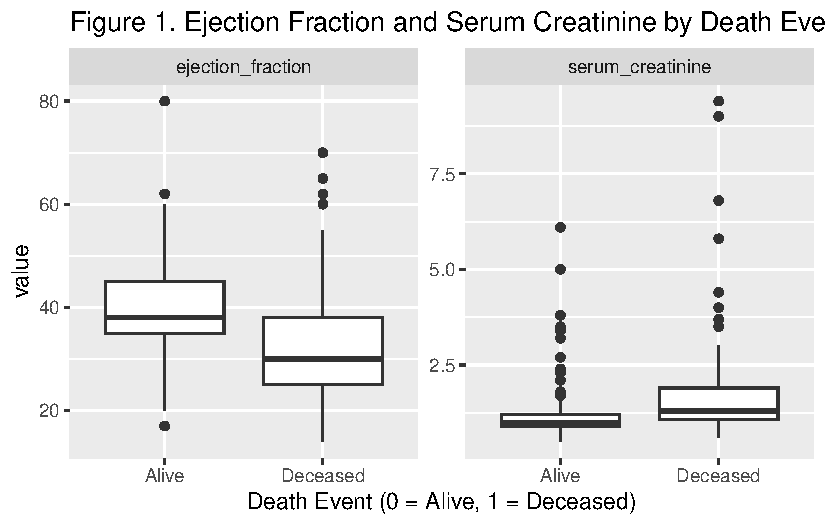
\includegraphics{SDS-291-final-project-report_files/figure-pdf/unnamed-chunk-7-1.pdf}

}

\end{figure}

\hypertarget{select-variables}{%
\subsubsection{Select variables}\label{select-variables}}

\begin{Shaded}
\begin{Highlighting}[]
\CommentTok{\# Selecting variables by doing backward elimination using nested F test (p{-}value = 0.1)}

\NormalTok{heart\_full }\OtherTok{\textless{}{-}} \FunctionTok{glm}\NormalTok{(DEATH\_EVENT }\SpecialCharTok{\textasciitilde{}}\NormalTok{ age }\SpecialCharTok{+}\NormalTok{ anaemia }\SpecialCharTok{+}\NormalTok{ creatinine\_phosphokinase }\SpecialCharTok{+}\NormalTok{ diabetes }\SpecialCharTok{+}\NormalTok{ ejection\_fraction }\SpecialCharTok{+}\NormalTok{ high\_blood\_pressure }\SpecialCharTok{+}\NormalTok{ platelets }\SpecialCharTok{+}\NormalTok{ serum\_creatinine }\SpecialCharTok{+}\NormalTok{ serum\_sodium }\SpecialCharTok{+}\NormalTok{ sex }\SpecialCharTok{+}\NormalTok{ smoking }\SpecialCharTok{+}\NormalTok{ time, }\AttributeTok{data =}\NormalTok{ heart\_data, }\AttributeTok{family =} \StringTok{"binomial"}\NormalTok{)}

\CommentTok{\# drop1(heart\_full, test = "F")}
\NormalTok{drop1\_heart }\OtherTok{\textless{}{-}} \FunctionTok{update}\NormalTok{(heart\_full, . }\SpecialCharTok{\textasciitilde{}}\NormalTok{ . }\SpecialCharTok{{-}}\NormalTok{ anaemia)}
\CommentTok{\# drop1(drop1\_heart, test = "F")}
\NormalTok{drop1\_heart }\OtherTok{\textless{}{-}} \FunctionTok{update}\NormalTok{(drop1\_heart, . }\SpecialCharTok{\textasciitilde{}}\NormalTok{ . }\SpecialCharTok{{-}}\NormalTok{ smoking)}
\CommentTok{\# drop1(drop1\_heart, test = "F")}
\NormalTok{drop1\_heart }\OtherTok{\textless{}{-}} \FunctionTok{update}\NormalTok{(drop1\_heart, . }\SpecialCharTok{\textasciitilde{}}\NormalTok{ . }\SpecialCharTok{{-}}\NormalTok{ high\_blood\_pressure)}
\CommentTok{\# drop1(drop1\_heart, test = "F")}
\NormalTok{drop1\_heart }\OtherTok{\textless{}{-}} \FunctionTok{update}\NormalTok{(drop1\_heart, . }\SpecialCharTok{\textasciitilde{}}\NormalTok{ . }\SpecialCharTok{{-}}\NormalTok{ diabetes)}
\CommentTok{\#  drop1(drop1\_heart, test = "F")}
\NormalTok{drop1\_heart }\OtherTok{\textless{}{-}} \FunctionTok{update}\NormalTok{(drop1\_heart, . }\SpecialCharTok{\textasciitilde{}}\NormalTok{ . }\SpecialCharTok{{-}}\NormalTok{ platelets)}
\CommentTok{\#  drop1(drop1\_heart, test = "F")}
\NormalTok{drop1\_heart }\OtherTok{\textless{}{-}} \FunctionTok{update}\NormalTok{(drop1\_heart, . }\SpecialCharTok{\textasciitilde{}}\NormalTok{ . }\SpecialCharTok{{-}}\NormalTok{ creatinine\_phosphokinase)}
\CommentTok{\# drop1(drop1\_heart, test = "F")}
\NormalTok{drop1\_heart }\OtherTok{\textless{}{-}} \FunctionTok{update}\NormalTok{(drop1\_heart, . }\SpecialCharTok{\textasciitilde{}}\NormalTok{ . }\SpecialCharTok{{-}}\NormalTok{ sex)}
\CommentTok{\# drop1(drop1\_heart, test = "F")}

\CommentTok{\# Final model after moving variables}
\NormalTok{final\_model }\OtherTok{\textless{}{-}}\NormalTok{ drop1\_heart}

\NormalTok{final\_model\_table }\OtherTok{\textless{}{-}} \FunctionTok{summary}\NormalTok{(final\_model)}\SpecialCharTok{$}\NormalTok{coefficients}
\NormalTok{final\_model\_table }\SpecialCharTok{|\textgreater{}} 
  \FunctionTok{kbl}\NormalTok{(}\AttributeTok{col.names =} \FunctionTok{c}\NormalTok{(}\StringTok{"Estimate"}\NormalTok{, }\StringTok{"Std. Error"}\NormalTok{, }\StringTok{"t value"}\NormalTok{, }\StringTok{"Pr(\textgreater{}|t|)"}\NormalTok{), }
      \AttributeTok{align =} \StringTok{"c"}\NormalTok{,}
      \AttributeTok{booktabs =} \ConstantTok{TRUE}\NormalTok{,}
      \AttributeTok{linesep =} \StringTok{""}\NormalTok{,}
      \AttributeTok{digits =} \FunctionTok{c}\NormalTok{(}\DecValTok{4}\NormalTok{, }\DecValTok{4}\NormalTok{, }\DecValTok{4}\NormalTok{, }\DecValTok{5}\NormalTok{),}
      \AttributeTok{caption =} \StringTok{"Coefficient Estimates from Final Model"}\NormalTok{) }\SpecialCharTok{|\textgreater{}}
  \FunctionTok{kable\_classic}\NormalTok{(}\AttributeTok{full\_width =} \ConstantTok{FALSE}\NormalTok{, }\AttributeTok{latex\_options =} \FunctionTok{c}\NormalTok{(}\StringTok{"HOLD\_position"}\NormalTok{))}
\end{Highlighting}
\end{Shaded}

\begin{table}[H]
\centering
\caption{Coefficient Estimates from Final Model}
\centering
\begin{tabular}[t]{lcccc}
\toprule
  & Estimate & Std. Error & t value & Pr(>|t|)\\
\midrule
(Intercept) & 9.4930 & 5.4058 & 1.7561 & 0.07907\\
age & 0.0425 & 0.0150 & 2.8255 & 0.00472\\
ejection\_fraction & -0.0734 & 0.0158 & -4.6518 & 0.00000\\
serum\_creatinine & 0.6860 & 0.1740 & 3.9415 & 0.00008\\
serum\_sodium & -0.0646 & 0.0384 & -1.6822 & 0.09254\\
time & -0.0209 & 0.0029 & -7.1657 & 0.00000\\
\bottomrule
\end{tabular}
\end{table}

\hypertarget{model-diagnose}{%
\subsubsection{Model diagnose}\label{model-diagnose}}

\begin{Shaded}
\begin{Highlighting}[]
\CommentTok{\# Model diagnostics}
\CommentTok{\# Cooks Distance}


\CommentTok{\# Influential points}

\CommentTok{\# Leverage}
\NormalTok{case\_influence }\OtherTok{\textless{}{-}}\NormalTok{ final\_model }\SpecialCharTok{|\textgreater{}} \FunctionTok{augment}\NormalTok{()}
\NormalTok{case\_influence }\OtherTok{\textless{}{-}}\NormalTok{ case\_influence }\SpecialCharTok{|\textgreater{}} \FunctionTok{mutate}\NormalTok{(}\AttributeTok{row\_id =} \FunctionTok{row\_number}\NormalTok{())}

\CommentTok{\# Calculating the threshold for unusually high leverage}
\NormalTok{k\_plus\_one }\OtherTok{\textless{}{-}} \FunctionTok{length}\NormalTok{(}\FunctionTok{coef}\NormalTok{(final\_model))}
\NormalTok{n }\OtherTok{\textless{}{-}} \FunctionTok{nrow}\NormalTok{(heart\_data)}

\CommentTok{\# Filtering the data to determine which observations have unusually high leverage}
\NormalTok{leverage\_index }\OtherTok{\textless{}{-}}\NormalTok{ case\_influence }\SpecialCharTok{|\textgreater{}} \FunctionTok{filter}\NormalTok{(.hat }\SpecialCharTok{\textgreater{}} \DecValTok{2} \SpecialCharTok{*}\NormalTok{ k\_plus\_one}\SpecialCharTok{/}\NormalTok{n) }\SpecialCharTok{|\textgreater{}} \FunctionTok{select}\NormalTok{(row\_id) }\SpecialCharTok{|\textgreater{}} \FunctionTok{pull}\NormalTok{()}
\NormalTok{heart\_data[leverage\_index, ]}
\end{Highlighting}
\end{Shaded}

\begin{verbatim}
    age anaemia creatinine_phosphokinase diabetes ejection_fraction
8    60       1                      315        1                60
9    65       0                      157        0                65
20   48       1                      582        1                55
24   53       0                       63        1                60
33   50       1                      249        1                35
37   90       1                       60        1                50
38   82       1                      855        1                50
53   60       0                     3964        1                62
67   42       1                      250        1                15
103  80       0                      898        0                25
111  85       0                      129        0                60
115  60       1                      754        1                40
118  85       1                      102        0                60
127  46       0                      168        1                17
130  53       1                      270        1                35
132  60       1                     1082        1                45
200  60       0                     1211        1                35
204  60       0                       59        0                25
218  54       1                      427        0                70
221  73       0                      582        0                20
229  65       0                       56        0                25
283  42       0                       64        0                30
    high_blood_pressure platelets serum_creatinine serum_sodium sex smoking
8                     0    454000             1.10          131   1       1
9                     0    263358             1.50          138   0       0
20                    0     87000             1.90          121   0       0
24                    0    368000             0.80          135   1       0
33                    1    319000             1.00          128   0       0
37                    0    226000             1.00          134   1       0
38                    1    321000             1.00          145   0       0
53                    0    263358             6.80          146   0       0
67                    0    213000             1.30          136   0       0
103                   0    149000             1.10          144   1       1
111                   0    306000             1.20          132   1       1
115                   1    328000             1.20          126   1       0
118                   0    507000             3.20          138   0       0
127                   1    271000             2.10          124   0       0
130                   0    227000             3.40          145   1       0
132                   0    250000             6.10          131   1       0
200                   0    263358             1.80          113   1       1
204                   1    212000             3.50          136   1       1
218                   1    151000             9.00          137   0       0
221                   0    263358             1.83          134   1       0
229                   0    237000             5.00          130   0       0
283                   0    215000             3.80          128   1       1
    time DEATH_EVENT
8     10    Deceased
9     10    Deceased
20    15    Deceased
24    22       Alive
33    28    Deceased
37    30    Deceased
38    30    Deceased
53    43    Deceased
67    65    Deceased
103   87       Alive
111   90    Deceased
115   91       Alive
118   94       Alive
127  100    Deceased
130  105       Alive
132  107       Alive
200  186       Alive
204  187       Alive
218  196    Deceased
221  198    Deceased
229  207       Alive
283  250       Alive
\end{verbatim}

\begin{Shaded}
\begin{Highlighting}[]
\NormalTok{case\_influence }\SpecialCharTok{|\textgreater{}} \FunctionTok{ggplot}\NormalTok{(}\FunctionTok{aes}\NormalTok{(}\AttributeTok{x =}\NormalTok{ row\_id, }\AttributeTok{y =}\NormalTok{ .hat)) }\SpecialCharTok{+} \FunctionTok{geom\_point}\NormalTok{() }\SpecialCharTok{+} 
  \FunctionTok{geom\_hline}\NormalTok{(}\AttributeTok{yintercept =} \DecValTok{2}\SpecialCharTok{*}\NormalTok{k\_plus\_one}\SpecialCharTok{/}\NormalTok{n, }\AttributeTok{col =} \StringTok{"red"}\NormalTok{) }\SpecialCharTok{+}
  \FunctionTok{xlab}\NormalTok{(}\StringTok{""}\NormalTok{) }\SpecialCharTok{+} \FunctionTok{ylab}\NormalTok{(}\StringTok{"Leverage"}\NormalTok{)}
\end{Highlighting}
\end{Shaded}

\begin{figure}[H]

{\centering 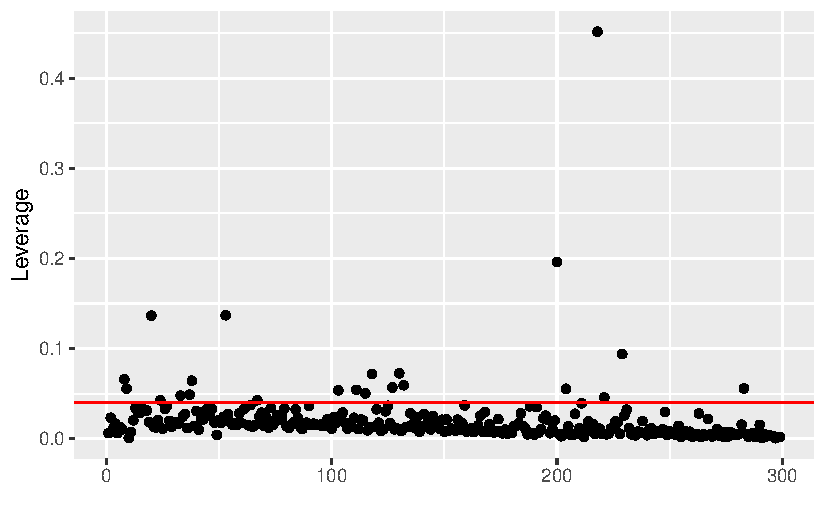
\includegraphics{SDS-291-final-project-report_files/figure-pdf/unnamed-chunk-9-1.pdf}

}

\end{figure}

\begin{Shaded}
\begin{Highlighting}[]
\CommentTok{\# Studentized residuals}
\NormalTok{case\_influence }\OtherTok{\textless{}{-}}\NormalTok{ case\_influence }\SpecialCharTok{|\textgreater{}} \FunctionTok{mutate}\NormalTok{(}\AttributeTok{.stu.resid =} \FunctionTok{rstudent}\NormalTok{(final\_model))}
\NormalTok{stu\_resid\_id }\OtherTok{\textless{}{-}}\NormalTok{ case\_influence }\SpecialCharTok{|\textgreater{}} \FunctionTok{filter}\NormalTok{(.stu.resid }\SpecialCharTok{\textless{}} \SpecialCharTok{{-}}\DecValTok{2} \SpecialCharTok{|}\NormalTok{ .stu.resid }\SpecialCharTok{\textgreater{}} \DecValTok{2}\NormalTok{) }\SpecialCharTok{|\textgreater{}} \FunctionTok{select}\NormalTok{(row\_id) }\SpecialCharTok{|\textgreater{}} \FunctionTok{pull}\NormalTok{()}
\NormalTok{heart\_data[stu\_resid\_id, ]}
\end{Highlighting}
\end{Shaded}

\begin{verbatim}
    age anaemia creatinine_phosphokinase diabetes ejection_fraction
21   65       1                       52        0                25
39   60       0                     2656        1                30
132  60       1                     1082        1                45
164  50       1                     2334        1                35
187  50       0                      582        0                50
196  77       1                      418        0                45
214  48       1                      131        1                30
247  55       0                     2017        0                25
263  65       1                      258        1                25
267  55       0                     1199        0                20
    high_blood_pressure platelets serum_creatinine serum_sodium sex smoking
21                    1    276000             1.30          137   0       0
39                    0    305000             2.30          137   1       0
132                   0    250000             6.10          131   1       0
164                   0     75000             0.90          142   0       0
187                   0    153000             0.60          134   0       0
196                   0    223000             1.80          145   1       0
214                   1    244000             1.60          130   0       0
247                   0    314000             1.10          138   1       0
263                   0    198000             1.40          129   1       0
267                   0    263358             1.83          134   1       1
    time DEATH_EVENT
21    16       Alive
39    30       Alive
132  107       Alive
164  126    Deceased
187  172    Deceased
196  180    Deceased
214  193    Deceased
247  214    Deceased
263  235    Deceased
267  241    Deceased
\end{verbatim}

\begin{Shaded}
\begin{Highlighting}[]
\CommentTok{\# Plotting the studentized residuals against the observation row numbers}
\NormalTok{case\_influence }\SpecialCharTok{|\textgreater{}}
  \FunctionTok{ggplot}\NormalTok{(}\FunctionTok{aes}\NormalTok{(}\AttributeTok{x =}\NormalTok{ row\_id, }\AttributeTok{y =}\NormalTok{ .stu.resid)) }\SpecialCharTok{+} \FunctionTok{geom\_point}\NormalTok{() }\SpecialCharTok{+} 
  \FunctionTok{geom\_hline}\NormalTok{(}\AttributeTok{yintercept =} \SpecialCharTok{{-}}\DecValTok{2}\NormalTok{, }\AttributeTok{col =} \StringTok{"red"}\NormalTok{) }\SpecialCharTok{+}
  \FunctionTok{geom\_hline}\NormalTok{(}\AttributeTok{yintercept =} \DecValTok{2}\NormalTok{, }\AttributeTok{col =} \StringTok{"red"}\NormalTok{) }\SpecialCharTok{+}
  \FunctionTok{xlab}\NormalTok{(}\StringTok{"Row ID"}\NormalTok{) }\SpecialCharTok{+} \FunctionTok{ylab}\NormalTok{(}\StringTok{"Studentized Residual"}\NormalTok{)}
\end{Highlighting}
\end{Shaded}

\begin{figure}[H]

{\centering 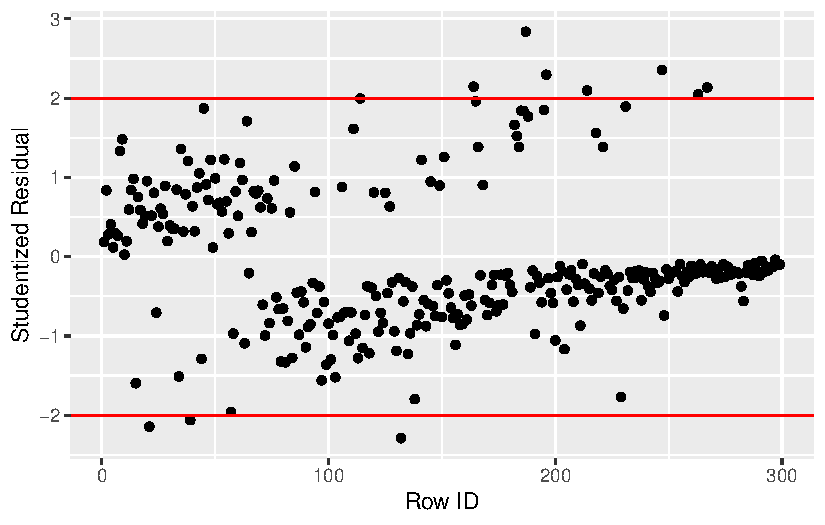
\includegraphics{SDS-291-final-project-report_files/figure-pdf/unnamed-chunk-9-2.pdf}

}

\end{figure}

\begin{Shaded}
\begin{Highlighting}[]
\CommentTok{\# Determining which observations have unusually large studentized residuals}
\NormalTok{stu\_resid\_id }\OtherTok{\textless{}{-}}\NormalTok{ case\_influence }\SpecialCharTok{|\textgreater{}}
  \FunctionTok{filter}\NormalTok{(.stu.resid }\SpecialCharTok{\textless{}} \SpecialCharTok{{-}}\DecValTok{2} \SpecialCharTok{|}\NormalTok{ .stu.resid }\SpecialCharTok{\textgreater{}} \DecValTok{2}\NormalTok{) }\SpecialCharTok{|\textgreater{}}
  \FunctionTok{select}\NormalTok{(row\_id) }\SpecialCharTok{|\textgreater{}}
  \FunctionTok{pull}\NormalTok{()}

\NormalTok{heart\_data[stu\_resid\_id, ]}
\end{Highlighting}
\end{Shaded}

\begin{verbatim}
    age anaemia creatinine_phosphokinase diabetes ejection_fraction
21   65       1                       52        0                25
39   60       0                     2656        1                30
132  60       1                     1082        1                45
164  50       1                     2334        1                35
187  50       0                      582        0                50
196  77       1                      418        0                45
214  48       1                      131        1                30
247  55       0                     2017        0                25
263  65       1                      258        1                25
267  55       0                     1199        0                20
    high_blood_pressure platelets serum_creatinine serum_sodium sex smoking
21                    1    276000             1.30          137   0       0
39                    0    305000             2.30          137   1       0
132                   0    250000             6.10          131   1       0
164                   0     75000             0.90          142   0       0
187                   0    153000             0.60          134   0       0
196                   0    223000             1.80          145   1       0
214                   1    244000             1.60          130   0       0
247                   0    314000             1.10          138   1       0
263                   0    198000             1.40          129   1       0
267                   0    263358             1.83          134   1       1
    time DEATH_EVENT
21    16       Alive
39    30       Alive
132  107       Alive
164  126    Deceased
187  172    Deceased
196  180    Deceased
214  193    Deceased
247  214    Deceased
263  235    Deceased
267  241    Deceased
\end{verbatim}

\begin{Shaded}
\begin{Highlighting}[]
\CommentTok{\# Cook\textquotesingle{}s distance}
\NormalTok{case\_influence }\SpecialCharTok{|\textgreater{}} \FunctionTok{select}\NormalTok{(.cooksd)}
\end{Highlighting}
\end{Shaded}

\begin{verbatim}
# A tibble: 299 x 1
        .cooksd
          <dbl>
 1 0.0000183   
 2 0.00167     
 3 0.0000777   
 4 0.000247    
 5 0.00000726  
 6 0.0000977   
 7 0.0000608   
 8 0.0166      
 9 0.0191      
10 0.0000000448
# i 289 more rows
\end{verbatim}

\begin{Shaded}
\begin{Highlighting}[]
\NormalTok{case\_influence }\SpecialCharTok{|\textgreater{}} \FunctionTok{filter}\NormalTok{(.cooksd }\SpecialCharTok{\textgreater{}} \FloatTok{0.05}\NormalTok{)}
\end{Highlighting}
\end{Shaded}

\begin{verbatim}
# A tibble: 3 x 14
  DEATH_EVENT   age ejection_fraction serum_creatinine serum_sodium  time
  <fct>       <dbl>             <int>            <dbl>        <int> <int>
1 Alive          60                45              6.1          131   107
2 Deceased       54                70              9            137   196
3 Alive          65                25              5            130   207
# i 8 more variables: .fitted <dbl>, .resid <dbl>, .hat <dbl>, .sigma <dbl>,
#   .cooksd <dbl>, .std.resid <dbl>, row_id <int>, .stu.resid <dbl>
\end{verbatim}

\begin{Shaded}
\begin{Highlighting}[]
\NormalTok{cooksd\_id }\OtherTok{\textless{}{-}}\NormalTok{ case\_influence }\SpecialCharTok{|\textgreater{}} \FunctionTok{filter}\NormalTok{(.cooksd }\SpecialCharTok{\textgreater{}} \FloatTok{0.05}\NormalTok{) }\SpecialCharTok{|\textgreater{}} \FunctionTok{select}\NormalTok{(row\_id) }\SpecialCharTok{|\textgreater{}} \FunctionTok{pull}\NormalTok{()}
\NormalTok{heart\_data[cooksd\_id, ]}
\end{Highlighting}
\end{Shaded}

\begin{verbatim}
    age anaemia creatinine_phosphokinase diabetes ejection_fraction
132  60       1                     1082        1                45
218  54       1                      427        0                70
229  65       0                       56        0                25
    high_blood_pressure platelets serum_creatinine serum_sodium sex smoking
132                   0    250000              6.1          131   1       0
218                   1    151000              9.0          137   0       0
229                   0    237000              5.0          130   0       0
    time DEATH_EVENT
132  107       Alive
218  196    Deceased
229  207       Alive
\end{verbatim}

\begin{Shaded}
\begin{Highlighting}[]
\CommentTok{\# Plotting the Cook\textquotesingle{}s distances against the observation row numbers}
\NormalTok{case\_influence }\SpecialCharTok{|\textgreater{}}
  \FunctionTok{ggplot}\NormalTok{(}\FunctionTok{aes}\NormalTok{(}\AttributeTok{x =}\NormalTok{ row\_id, }\AttributeTok{y =}\NormalTok{ .cooksd)) }\SpecialCharTok{+}
  \FunctionTok{geom\_point}\NormalTok{() }\SpecialCharTok{+} 
  \FunctionTok{geom\_hline}\NormalTok{(}\AttributeTok{yintercept =} \FloatTok{0.05}\NormalTok{, }\AttributeTok{col =} \StringTok{"red"}\NormalTok{) }\SpecialCharTok{+}
  \FunctionTok{xlab}\NormalTok{(}\StringTok{"Row ID"}\NormalTok{) }\SpecialCharTok{+} \FunctionTok{ylab}\NormalTok{(}\StringTok{"Cook\textquotesingle{}s Distance"}\NormalTok{)}
\end{Highlighting}
\end{Shaded}

\begin{figure}[H]

{\centering 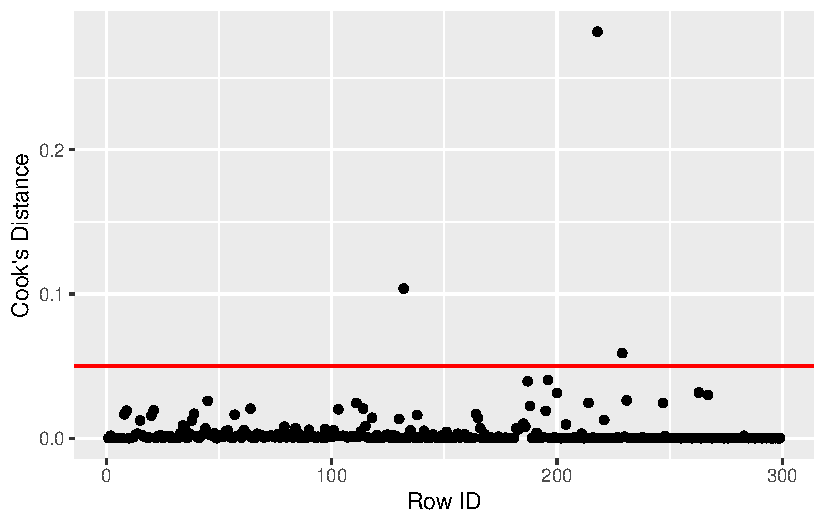
\includegraphics{SDS-291-final-project-report_files/figure-pdf/unnamed-chunk-9-3.pdf}

}

\end{figure}

\begin{Shaded}
\begin{Highlighting}[]
\CommentTok{\# Define the row indices of the influential observations}
\NormalTok{influential\_rows }\OtherTok{\textless{}{-}} \FunctionTok{c}\NormalTok{(}\DecValTok{132}\NormalTok{, }\DecValTok{218}\NormalTok{, }\DecValTok{229}\NormalTok{)}

\CommentTok{\# Remove these rows from the heart\_data dataset}
\NormalTok{heart\_data\_clean }\OtherTok{\textless{}{-}}\NormalTok{ heart\_data[}\SpecialCharTok{{-}}\NormalTok{influential\_rows, ]}

\CommentTok{\# Refit the logistic regression model on the cleaned data}
\NormalTok{final\_model\_clean }\OtherTok{\textless{}{-}} \FunctionTok{glm}\NormalTok{(DEATH\_EVENT }\SpecialCharTok{\textasciitilde{}}\NormalTok{ age }\SpecialCharTok{+}\NormalTok{ anaemia }\SpecialCharTok{+}\NormalTok{ creatinine\_phosphokinase }\SpecialCharTok{+}\NormalTok{ diabetes }\SpecialCharTok{+}\NormalTok{ ejection\_fraction }\SpecialCharTok{+}\NormalTok{ high\_blood\_pressure }\SpecialCharTok{+}\NormalTok{ platelets }\SpecialCharTok{+}\NormalTok{ serum\_creatinine }\SpecialCharTok{+}\NormalTok{ serum\_sodium }\SpecialCharTok{+}\NormalTok{ sex }\SpecialCharTok{+}\NormalTok{ smoking }\SpecialCharTok{+}\NormalTok{ time, }\AttributeTok{data =}\NormalTok{ heart\_data\_clean, }\AttributeTok{family =} \StringTok{"binomial"}\NormalTok{)}

\CommentTok{\# Summarize the new model}
\FunctionTok{summary}\NormalTok{(final\_model\_clean)}
\end{Highlighting}
\end{Shaded}

\begin{verbatim}

Call:
glm(formula = DEATH_EVENT ~ age + anaemia + creatinine_phosphokinase + 
    diabetes + ejection_fraction + high_blood_pressure + platelets + 
    serum_creatinine + serum_sodium + sex + smoking + time, family = "binomial", 
    data = heart_data_clean)

Coefficients:
                           Estimate Std. Error z value Pr(>|z|)    
(Intercept)               1.169e+01  5.895e+00   1.984  0.04727 *  
age                       4.913e-02  1.642e-02   2.993  0.00276 ** 
anaemia1                  3.327e-03  3.739e-01   0.009  0.99290    
creatinine_phosphokinase  2.349e-04  1.844e-04   1.273  0.20285    
diabetes1                 2.052e-01  3.597e-01   0.570  0.56847    
ejection_fraction        -8.256e-02  1.775e-02  -4.652 3.28e-06 ***
high_blood_pressure1     -2.114e-01  3.749e-01  -0.564  0.57286    
platelets                -1.010e-06  1.928e-06  -0.524  0.60038    
serum_creatinine          8.737e-01  2.931e-01   2.981  0.00287 ** 
serum_sodium             -7.895e-02  4.104e-02  -1.924  0.05439 .  
sex1                     -5.389e-01  4.266e-01  -1.263  0.20659    
smoking1                 -6.404e-02  4.229e-01  -0.151  0.87963    
time                     -2.144e-02  3.126e-03  -6.860 6.88e-12 ***
---
Signif. codes:  0 '***' 0.001 '**' 0.01 '*' 0.05 '.' 0.1 ' ' 1

(Dispersion parameter for binomial family taken to be 1)

    Null deviance: 371.53  on 295  degrees of freedom
Residual deviance: 209.31  on 283  degrees of freedom
AIC: 235.31

Number of Fisher Scoring iterations: 6
\end{verbatim}

\begin{Shaded}
\begin{Highlighting}[]
\CommentTok{\# Multicollinearity}
\FunctionTok{vif}\NormalTok{(final\_model)}
\end{Highlighting}
\end{Shaded}

\begin{verbatim}
              age ejection_fraction  serum_creatinine      serum_sodium 
         1.053111          1.133484          1.079122          1.028355 
             time 
         1.096862 
\end{verbatim}

\begin{Shaded}
\begin{Highlighting}[]
\CommentTok{\# Checking conditions using Deviance residual plot}
\FunctionTok{plot}\NormalTok{(}\FunctionTok{residuals}\NormalTok{(final\_model, }\AttributeTok{type =} \StringTok{"deviance"}\NormalTok{), }\AttributeTok{ylab =} \StringTok{"Deviance Residuals"}\NormalTok{)}
\end{Highlighting}
\end{Shaded}

\begin{figure}[H]

{\centering 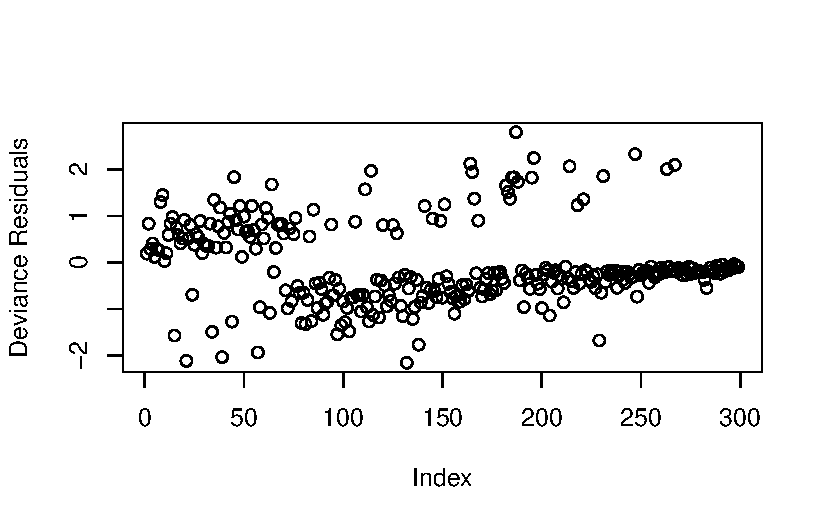
\includegraphics{SDS-291-final-project-report_files/figure-pdf/unnamed-chunk-9-4.pdf}

}

\end{figure}

\hypertarget{model-performance-1}{%
\subsubsection{Model performance}\label{model-performance-1}}

\begin{Shaded}
\begin{Highlighting}[]
\NormalTok{new\_data }\OtherTok{\textless{}{-}} \FunctionTok{read.csv}\NormalTok{(}\StringTok{"heart\_failure\_clinical\_records\_dataset.csv"}\NormalTok{)}
\NormalTok{new\_data}\SpecialCharTok{$}\NormalTok{anaemia }\OtherTok{\textless{}{-}} \FunctionTok{factor}\NormalTok{(new\_data}\SpecialCharTok{$}\NormalTok{anaemia)}
\NormalTok{new\_data}\SpecialCharTok{$}\NormalTok{diabetes }\OtherTok{\textless{}{-}} \FunctionTok{factor}\NormalTok{(new\_data}\SpecialCharTok{$}\NormalTok{diabetes)}
\NormalTok{new\_data}\SpecialCharTok{$}\NormalTok{high\_blood\_pressure }\OtherTok{\textless{}{-}} \FunctionTok{factor}\NormalTok{(new\_data}\SpecialCharTok{$}\NormalTok{high\_blood\_pressure)}
\NormalTok{new\_data}\SpecialCharTok{$}\NormalTok{sex }\OtherTok{\textless{}{-}} \FunctionTok{factor}\NormalTok{(new\_data}\SpecialCharTok{$}\NormalTok{sex)}
\NormalTok{new\_data}\SpecialCharTok{$}\NormalTok{smoking }\OtherTok{\textless{}{-}} \FunctionTok{factor}\NormalTok{(new\_data}\SpecialCharTok{$}\NormalTok{smoking)}
\NormalTok{new\_data}\SpecialCharTok{$}\NormalTok{DEATH\_EVENT }\OtherTok{\textless{}{-}} \FunctionTok{factor}\NormalTok{(new\_data}\SpecialCharTok{$}\NormalTok{DEATH\_EVENT, }\AttributeTok{levels =} \FunctionTok{c}\NormalTok{(}\DecValTok{0}\NormalTok{,}\DecValTok{1}\NormalTok{), }
                         \AttributeTok{labels =} \FunctionTok{c}\NormalTok{(}\StringTok{"Alive"}\NormalTok{, }\StringTok{"Deceased"}\NormalTok{))}

\CommentTok{\# Get predicted probabilities for new data}
\NormalTok{new\_pred }\OtherTok{\textless{}{-}} \FunctionTok{augment}\NormalTok{(final\_model, }\AttributeTok{newdata =}\NormalTok{ new\_data, }\AttributeTok{type.predict =} \StringTok{"response"}\NormalTok{)}

\CommentTok{\# Classify using 0.3 threshold}
\NormalTok{new\_classify }\OtherTok{\textless{}{-}}\NormalTok{ new\_pred }\SpecialCharTok{|\textgreater{}}
  \FunctionTok{mutate}\NormalTok{(}\AttributeTok{pred =} \FunctionTok{ifelse}\NormalTok{(.fitted }\SpecialCharTok{\textgreater{}} \FloatTok{0.3}\NormalTok{, }\StringTok{"Deceased"}\NormalTok{, }\StringTok{"Alive"}\NormalTok{))}

\CommentTok{\# Actual vs. Predicted table with margins}
\NormalTok{compare\_table }\OtherTok{\textless{}{-}}\NormalTok{ new\_classify }\SpecialCharTok{|\textgreater{}}
  \FunctionTok{select}\NormalTok{(DEATH\_EVENT, pred) }\SpecialCharTok{|\textgreater{}}
  \FunctionTok{table}\NormalTok{() }\SpecialCharTok{|\textgreater{}}
  \FunctionTok{addmargins}\NormalTok{()}

\CommentTok{\# Calculate sensitivity, specificity, accuracy}
\NormalTok{sensitivity }\OtherTok{\textless{}{-}}\NormalTok{ compare\_table[}\DecValTok{2}\NormalTok{, }\DecValTok{2}\NormalTok{] }\SpecialCharTok{/}\NormalTok{ compare\_table[}\DecValTok{2}\NormalTok{, }\DecValTok{3}\NormalTok{]}
\NormalTok{specificity }\OtherTok{\textless{}{-}}\NormalTok{ compare\_table[}\DecValTok{1}\NormalTok{, }\DecValTok{1}\NormalTok{] }\SpecialCharTok{/}\NormalTok{ compare\_table[}\DecValTok{1}\NormalTok{, }\DecValTok{3}\NormalTok{]}
\NormalTok{accuracy }\OtherTok{\textless{}{-}}\NormalTok{ (compare\_table[}\DecValTok{1}\NormalTok{, }\DecValTok{1}\NormalTok{] }\SpecialCharTok{+}\NormalTok{ compare\_table[}\DecValTok{2}\NormalTok{, }\DecValTok{2}\NormalTok{]) }\SpecialCharTok{/}\NormalTok{ compare\_table[}\DecValTok{3}\NormalTok{, }\DecValTok{3}\NormalTok{]}


\CommentTok{\# Create ROC object}
\NormalTok{voting\_roc }\OtherTok{\textless{}{-}} \FunctionTok{roc}\NormalTok{(}
  \AttributeTok{response =}\NormalTok{ new\_classify}\SpecialCharTok{$}\NormalTok{DEATH\_EVENT,}
  \AttributeTok{predictor =}\NormalTok{ new\_classify}\SpecialCharTok{$}\NormalTok{.fitted,}
  \AttributeTok{quiet =} \ConstantTok{TRUE}
\NormalTok{)}

\CommentTok{\# Calculate AUC}
\NormalTok{auc\_value }\OtherTok{\textless{}{-}} \FunctionTok{auc}\NormalTok{(voting\_roc)}

\CommentTok{\# Results}
\FunctionTok{cat}\NormalTok{(}\StringTok{"Sensitivity:"}\NormalTok{, sensitivity, }\StringTok{"}\SpecialCharTok{\textbackslash{}n}\StringTok{"}\NormalTok{)}
\end{Highlighting}
\end{Shaded}

\begin{verbatim}
Sensitivity: 0.8125 
\end{verbatim}

\begin{Shaded}
\begin{Highlighting}[]
\FunctionTok{cat}\NormalTok{(}\StringTok{"Specificity:"}\NormalTok{, specificity, }\StringTok{"}\SpecialCharTok{\textbackslash{}n}\StringTok{"}\NormalTok{)}
\end{Highlighting}
\end{Shaded}

\begin{verbatim}
Specificity: 0.7931034 
\end{verbatim}

\begin{Shaded}
\begin{Highlighting}[]
\FunctionTok{cat}\NormalTok{(}\StringTok{"Accuracy:"}\NormalTok{, accuracy, }\StringTok{"}\SpecialCharTok{\textbackslash{}n}\StringTok{"}\NormalTok{)}
\end{Highlighting}
\end{Shaded}

\begin{verbatim}
Accuracy: 0.7993311 
\end{verbatim}

\begin{Shaded}
\begin{Highlighting}[]
\FunctionTok{cat}\NormalTok{(}\StringTok{"AUC:"}\NormalTok{, auc\_value, }\StringTok{"}\SpecialCharTok{\textbackslash{}n}\StringTok{"}\NormalTok{)}
\end{Highlighting}
\end{Shaded}

\begin{verbatim}
AUC: 0.8935242 
\end{verbatim}

\hypertarget{results-section}{%
\subsubsection{Results section}\label{results-section}}

\begin{Shaded}
\begin{Highlighting}[]
\NormalTok{broom}\SpecialCharTok{::}\FunctionTok{tidy}\NormalTok{(final\_model, }\AttributeTok{conf.int =} \ConstantTok{TRUE}\NormalTok{, }\AttributeTok{exponentiate =} \ConstantTok{TRUE}\NormalTok{) }\SpecialCharTok{\%\textgreater{}\%}
  \FunctionTok{filter}\NormalTok{(term }\SpecialCharTok{!=} \StringTok{"(Intercept)"}\NormalTok{) }\SpecialCharTok{\%\textgreater{}\%}
\FunctionTok{mutate}\NormalTok{(}\AttributeTok{term =}\NormalTok{ dplyr}\SpecialCharTok{::}\FunctionTok{recode}\NormalTok{(term,}
  \StringTok{"age"} \OtherTok{=} \StringTok{"Age"}\NormalTok{,}
  \StringTok{"ejection\_fraction"} \OtherTok{=} \StringTok{"Ejection Fraction"}\NormalTok{,}
  \StringTok{"serum\_creatinine"} \OtherTok{=} \StringTok{"Serum Creatinine"}\NormalTok{,}
  \StringTok{"serum\_sodium"} \OtherTok{=} \StringTok{"Serum Sodium"}\NormalTok{,}
  \StringTok{"time"} \OtherTok{=} \StringTok{"Follow{-}up Time"}
\NormalTok{)) }\SpecialCharTok{\%\textgreater{}\%}
  \FunctionTok{select}\NormalTok{(term, estimate, conf.low, conf.high, p.value) }\SpecialCharTok{\%\textgreater{}\%}
\NormalTok{  knitr}\SpecialCharTok{::}\FunctionTok{kable}\NormalTok{(}
    \AttributeTok{col.names =} \FunctionTok{c}\NormalTok{(}\StringTok{"Predictor"}\NormalTok{, }\StringTok{"Odds Ratio"}\NormalTok{, }\StringTok{"95\% CI (Low)"}\NormalTok{, }\StringTok{"95\% CI (High)"}\NormalTok{, }\StringTok{"p{-}value"}\NormalTok{),}
    \AttributeTok{digits =} \DecValTok{3}\NormalTok{,}
    \AttributeTok{booktabs =} \ConstantTok{TRUE}\NormalTok{,}
    \AttributeTok{caption =} \StringTok{"Final Model: Odds Ratios and 95}\SpecialCharTok{\textbackslash{}\textbackslash{}}\StringTok{\% Confidence Intervals"}
\NormalTok{  ) }\SpecialCharTok{\%\textgreater{}\%}
  \FunctionTok{kable\_classic}\NormalTok{(}\AttributeTok{full\_width =} \ConstantTok{FALSE}\NormalTok{, }\AttributeTok{latex\_options =} \StringTok{"HOLD\_position"}\NormalTok{)}
\end{Highlighting}
\end{Shaded}

\begin{longtable}[t]{lrrrr}
\caption{Final Model: Odds Ratios and 95\% Confidence Intervals}\\
\toprule
Predictor & Odds Ratio & 95\% CI (Low) & 95\% CI (High) & p-value\\
\midrule
Age & 1.043 & 1.014 & 1.076 & 0.005\\
Ejection Fraction & 0.929 & 0.899 & 0.957 & 0.000\\
Serum Creatinine & 1.986 & 1.421 & 2.874 & 0.000\\
Serum Sodium & 0.937 & 0.868 & 1.011 & 0.093\\
Follow-up Time & 0.979 & 0.973 & 0.985 & 0.000\\
\bottomrule
\end{longtable}

\hypertarget{refs}{}
\begin{CSLReferences}{1}{0}
\leavevmode\vadjust pre{\hypertarget{ref-ahmad2018}{}}%
Ahmad, T., Lund, L. H., Rao, P., Ghosh, R., Warier, P., Vaccaro, B.,
Dahlström, U., O'Connor, C. M., Felker, G. M., Desai, N. R., et al.
(2018). Machine learning methods improve prognostication, identify
clinically distinct phenotypes, and detect heterogeneity in response to
therapy in a large cohort of heart failure patients. \emph{Journal of
the American Heart Association}, \emph{7}(8), e008081.
\url{https://doi.org/10.1161/JAHA.117.008081}

\leavevmode\vadjust pre{\hypertarget{ref-choi2017}{}}%
Choi, E., \& Lee, J. (2017). Predicting mortality in heart failure
patients with reduced or mildly reduced ejection fraction. \emph{Journal
of Cardiovascular Ultrasound}, \emph{25}(1), 1--10.
\url{https://doi.org/10.4250/jcu.2017.25.1.1}

\leavevmode\vadjust pre{\hypertarget{ref-savarese2017}{}}%
Savarese, G., \& Lund, L. H. (2017). Global public health burden of
heart failure. \emph{Cardiac Failure Review}, \emph{3}(1), 7--11.
\url{https://doi.org/10.15420/cfr.2016:25:2}

\leavevmode\vadjust pre{\hypertarget{ref-sulaiman2020}{}}%
Sulaiman, N., Chen, W., et al. (2020). Serum sodium as a predictor of
outcomes in heart failure: A review of the evidence. \emph{Heart and
Lung}, \emph{49}(5), 430--436.
\url{https://doi.org/10.1016/j.hrtlng.2020.05.001}

\end{CSLReferences}



\end{document}
